\iffalse
\documentclass[journal,12pt,twocolumn]{IEEEtran}
%
\usepackage{setspace}
\usepackage{gensymb}
\usepackage{xcolor}
\usepackage{caption}
%\usepackage{subcaption}
%\doublespacing
\singlespacing

%\usepackage{graphicx}
%\usepackage{amssymb}
%\usepackage{relsize}
\usepackage[cmex10]{amsmath}
\usepackage{mathtools}
%\usepackage{amsthm}
%\interdisplaylinepenalty=2500
%\savesymbol{iint}
%\usepackage{txfonts}
%\restoresymbol{TXF}{iint}
%\usepackage{wasysym}
\usepackage{hyperref}
\usepackage{amsthm}
\usepackage{mathrsfs}
\usepackage{txfonts}
\usepackage{stfloats}
\usepackage{cite}
\usepackage{cases}
\usepackage{subfig}
%\usepackage{xtab}
\usepackage{longtable}
\usepackage{multirow}
%\usepackage{algorithm}
%\usepackage{algpseudocode}
%\usepackage{enumerate}
\usepackage{enumitem}
\usepackage{mathtools}
%\usepackage{iithtlc}
%\usepackage[framemethod=tikz]{mdframed}
\usepackage{listings}
\let\vec\mathbf


%\usepackage{stmaryrd}


%\usepackage{wasysym}
%\newcounter{MYtempeqncnt}
\DeclareMathOperator*{\Res}{Res}
%\renewcommand{\baselinestretch}{2}
\renewcommand\thesection{\arabic{section}}
\renewcommand\thesubsection{\thesection.\arabic{subsection}}
\renewcommand\thesubsubsection{\thesubsection.\arabic{subsubsection}}

\renewcommand\thesectiondis{\arabic{section}}
\renewcommand\thesubsectiondis{\thesectiondis.\arabic{subsection}}
\renewcommand\thesubsubsectiondis{\thesubsectiondis.\arabic{subsubsection}}

%\renewcommand{\labelenumi}{\textbf{\theenumi}}
%\renewcommand{\theenumi}{P.\arabic{enumi}}

% correct bad hyphenation here
\hyphenation{op-tical net-works semi-conduc-tor}

\lstset{
language=Python,
frame=single, 
breaklines=true,
columns=fullflexible
}



\begin{document}
%

\theoremstyle{definition}
\newtheorem{theorem}{Theorem}[section]
\newtheorem{problem}{Problem}
\newtheorem{proposition}{Proposition}[section]
\newtheorem{lemma}{Lemma}[section]
\newtheorem{corollary}[theorem]{Corollary}
\newtheorem{example}{Example}[section]
\newtheorem{definition}{Definition}[section]
%\newtheorem{algorithm}{Algorithm}[section]
%\newtheorem{cor}{Corollary}
\newcommand{\BEQA}{\begin{eqnarray}}
\newcommand{\EEQA}{\end{eqnarray}}
\newcommand{\define}{\stackrel{\triangle}{=}}
\newcommand{\myvec}[1]{\ensuremath{\begin{pmatrix}#1\end{pmatrix}}}
\newcommand{\mydet}[1]{\ensuremath{\begin{vmatrix}#1\end{vmatrix}}}

\bibliographystyle{IEEEtran}
%\bibliographystyle{ieeetr}

\providecommand{\nCr}[2]{\,^{#1}C_{#2}} % nCr
\providecommand{\nPr}[2]{\,^{#1}P_{#2}} % nPr
\providecommand{\mbf}{\mathbf}
\providecommand{\pr}[1]{\ensuremath{\Pr\left(#1\right)}}
\providecommand{\qfunc}[1]{\ensuremath{Q\left(#1\right)}}
\providecommand{\sbrak}[1]{\ensuremath{{}\left[#1\right]}}
\providecommand{\lsbrak}[1]{\ensuremath{{}\left[#1\right.}}
\providecommand{\rsbrak}[1]{\ensuremath{{}\left.#1\right]}}
\providecommand{\brak}[1]{\ensuremath{\left(#1\right)}}
\providecommand{\lbrak}[1]{\ensuremath{\left(#1\right.}}
\providecommand{\rbrak}[1]{\ensuremath{\left.#1\right)}}
\providecommand{\cbrak}[1]{\ensuremath{\left\{#1\right\}}}
\providecommand{\lcbrak}[1]{\ensuremath{\left\{#1\right.}}
\providecommand{\rcbrak}[1]{\ensuremath{\left.#1\right\}}}
\theoremstyle{remark}
\newtheorem{rem}{Remark}
\newcommand{\sgn}{\mathop{\mathrm{sgn}}}
\providecommand{\abs}[1]{\left\vert#1\right\vert}
\providecommand{\res}[1]{\Res\displaylimits_{#1}} 
\providecommand{\norm}[1]{\lVert#1\rVert}
\providecommand{\mtx}[1]{\mathbf{#1}}
\providecommand{\mean}[1]{E\left[ #1 \right]}
\providecommand{\fourier}{\overset{\mathcal{F}}{ \rightleftharpoons}}
\providecommand{\ztrans}{\overset{\mathcal{Z}}{ \rightleftharpoons}}

%\providecommand{\hilbert}{\overset{\mathcal{H}}{ \rightleftharpoons}}
\providecommand{\system}{\overset{\mathcal{H}}{ \longleftrightarrow}}
	%\newcommand{\solution}[2]{\textbf{Solution:}{#1}}
\newcommand{\solution}{\noindent \textbf{Solution: }}
\providecommand{\dec}[2]{\ensuremath{\overset{#1}{\underset{#2}{\gtrless}}}}
\numberwithin{equation}{section}
%\numberwithin{equation}{subsection}
%\numberwithin{problem}{subsection}
%\numberwithin{definition}{subsection}

%\renewcommand{\thefigure}{\theproblem.\arabic{figure}}
\renewcommand{\thefigure}{\arabic{section}.\arabic{figure}}
\makeatletter
\@addtoreset{figure}{section}
\makeatother

%\numberwithin{figure}{subsection}

\def\putbox#1#2#3{\makebox[0in][l]{\makebox[#1][l]{}\raisebox{\baselineskip}[0in][0in]{\raisebox{#2}[0in][0in]{#3}}}}
     \def\rightbox#1{\makebox[0in][r]{#1}}
     \def\centbox#1{\makebox[0in]{#1}}
     \def\topbox#1{\raisebox{-\baselineskip}[0in][0in]{#1}}
     \def\midbox#1{\raisebox{-0.5\baselineskip}[0in][0in]{#1}}

\vspace{3cm}

\title{ 
%\logo{
%}
Pingala Series
%	\logo{Octave for Math Computing }
}
%\title{
%	\logo{Matrix Analysis through Octave}{\begin{center}\includegraphics[scale=.24]{tlc}\end{center}}{}{HAMDSP}
%}


% paper title
% can use linebreaks \\ within to get better formatting as desired
%\title{Matrix Analysis through Octave}
%
%
% author names and IEEE memberships
% note positions of commas and nonbreaking spaces ( ~ ) LaTeX will not break
% a structure at a ~ so this keeps an author's name from being broken across
% two lines.
% use \thanks{} to gain access to the first footnote area
% a separate \thanks must be used for each paragraph as LaTeX2e's \thanks
% was not built to handle multiple paragraphs
%

\author{Gautam Singh}
% note the % following the last \IEEEmembership and also \thanks - 
% these prevent an unwanted space from occurring between the last author name
% and the end of the author line. i.e., if you had this:
% 
% \author{....lastname \thanks{...} \thanks{...} }
%                     ^------------^------------^----Do not want these spaces!
%
% a space would be appended to the last name and could cause every name on that
% line to be shifted left slightly. This is one of those "LaTeX things". For
% instance, "\textbf{A} \textbf{B}" will typeset as "A B" not "AB". To get
% "AB" then you have to do: "\textbf{A}\textbf{B}"
% \thanks is no different in this regard, so shield the last } of each \thanks
% that ends a line with a % and do not let a space in before the next \thanks.
% Spaces after \IEEEmembership other than the last one are OK (and needed) as
% you are supposed to have spaces between the names. For what it is worth,
% this is a minor point as most people would not even notice if the said evil
% space somehow managed to creep in.



% The paper headers
%\markboth{Journal of \LaTeX\ Class Files,~Vol.~6, No.~1, January~2007}%
%{Shell \MakeLowercase{\textit{et al.}}: Bare Demo of IEEEtran.cls for Journals}
% The only time the second header will appear is for the odd numbered pages
% after the title page when using the twoside option.
% 
% *** Note that you probably will NOT want to include the author's ***
% *** name in the headers of peer review papers.                   ***
% You can use \ifCLASSOPTIONpeerreview for conditional compilation here if
% you desire.




% If you want to put a publisher's ID mark on the page you can do it like
% this:
%\IEEEpubid{0000--0000/00\$00.00~\copyright~2007 IEEE}
% Remember, if you use this you must call \IEEEpubidadjcol in the second
% column for its text to clear the IEEEpubid mark.



% make the title area
\maketitle

%\newpage

\tableofcontents

\bigskip

\begin{abstract}
This manual provides a simple introduction to Transforms
\end{abstract}
\fi
\section{JEE 2019}
\begin{align}
	\label{eq:pingala/10-orig-diff-a}
	a_n &= \frac{\alpha^{n}-\beta^{n}}{\alpha - \beta}, \quad n \ge 1
	\\
	b_n &= a_{n-1} + a_{n+1}, \quad n \ge 2, \quad b_1 =1
	\label{eq:pingala/10-orig-diff}
\end{align}
where $\alpha$ and $\beta$ ($\alpha > \beta$) are the roots of the
\begin{align}
z^2 - z - 1 = 0
\end{align}
%
Verify the following using a python code.
\begin{enumerate}[label=\thesection.\arabic*,ref=\thesection.\theenumi]
\item 
	\label{itm:ping-1}
\begin{align}
	\label{eq:ping-1}
	\sum_{k=1}^{n}a_k = a_{n+2}-1, \quad n \ge 1
\end{align}
 \item 
	\label{itm:ping-2}
\begin{align}
	\label{eq:ping-2}
	\sum_{k=1}^{\infty}\frac{a_k}{10^k} =\frac{10}{89}
\end{align}
 \item 
	\label{itm:ping-3}
\begin{align}
	\label{eq:ping-3}
	b_n =\alpha^n + \beta^n, \quad n \ge 1
\end{align}
 \item 
	\label{itm:ping-4}
\begin{align}
	\label{eq:ping-4}
	\sum_{k=1}^{\infty}\frac{b_k}{10^k} =\frac{8}{89}
\end{align}
\solution
\begin{lstlisting}
$ python3 pingala/codes/1.py
\end{lstlisting}
\end{enumerate}
\section{Pingala Series}
\begin{enumerate}[label=\thesection.\arabic*,ref=\thesection.\theenumi]
	\item The {\em Pingala} series is generated using the difference equation 
\begin{align}
	x(n+2) = x\brak{n+1} + x\brak{n},  \quad x(0) = x(1) = 1, n \ge 0
	\label{eq:pingala/10-pingala}
\end{align}
Generate a stem plot for $x(n)$.
\\
\solution
The following code generates
    Fig. \ref{fig:pingala/xn}.
\begin{lstlisting}
$ python3 pingala/codes/2_1.py
\end{lstlisting}
\begin{figure}[!htp]
    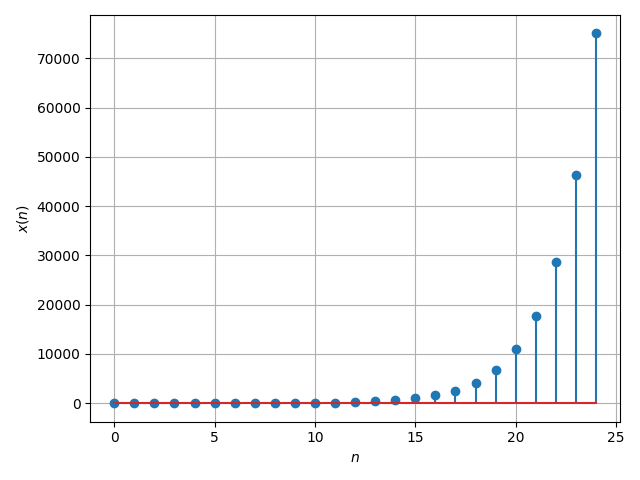
\includegraphics[width=\columnwidth]{pingala/figs/2_1.png}
    \caption{Plot of $x(n)$}
    \label{fig:pingala/xn}
\end{figure}
\item The {\em one sided} $Z$-transform of $x(n)$ is defined as 
\begin{align}
	X^{+}(z) = \sum_{n = 0}^{\infty}x(n)z^{-n}, \quad z \in \mathbb{C}
\label{eq:pingala/one-Z}
\end{align}
Find $X^{+}(z)$.
\\
\solution Taking the one-sided $Z$-transform on both sides of \eqref{eq:pingala/10-pingala},
\begin{align}
	\mathcal{Z}^+\sbrak{x(n + 2)} &= \mathcal{Z}^+\sbrak{x(n + 1)} + \mathcal{Z}^+\sbrak{x(n)} \\
\implies     z^2X^+(z) - z^2x(0) - zx(1) &= zX^+(z) - zx(0) + zX^+(z) \\
 \implies   \brak{z^2 - z - 1}X^+(z) &= z^2 \\
  \implies    X^+(z) = \frac{1}{1 - z^{-1} - z^{-2}} 
    &= \frac{1}{\brak{1 - \alpha z^{-1}}\brak{1 - \beta z^{-1}}}, \quad |z| > \alpha
    \label{eq:pingala/X-z}
\end{align}
\item Find $x(n)$.
\\
\solution Expanding $X^+(z)$ in \eqref{eq:pingala/X-z} using partial fractions, we get
\begin{align}
    X^+(z) &= \frac{1}{\brak{\alpha - \beta}}\sbrak{\frac{z}{1 - \alpha z^{-1}} - \frac{z}{1 - \beta z^{-1}}} \\
	\implies    x(n) &= \frac{\alpha^{n + 1} - \beta^{n + 1}}{\alpha - \beta}u(n) 
	\\
	&= a_{n + 1}
    \label{eq:pingala/x-n-def}
\end{align}
upon comparing with
	\eqref{eq:pingala/10-orig-diff-a}.
\end{enumerate}
\section{Linear Time Invariant System}
\begin{enumerate}[label=\thesection.\arabic*,ref=\thesection.\theenumi]
	\item Sketch 
\begin{align}
	y(n) = x\brak{n-1} + x\brak{n+1},  \quad n \ge 0
	\label{eq:pingala/10-orig-diff-rev}
\end{align}
\solution
Execute
\begin{lstlisting}
$ python3 pingala/codes/2_2.py
\end{lstlisting}
to obtain Fig. 
    \ref{fig:pingala/yn}
\begin{figure}[!htbp]
    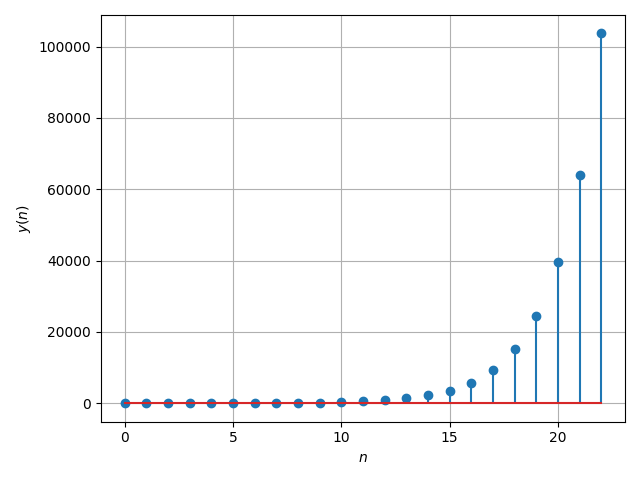
\includegraphics[width=\columnwidth]{pingala/figs/2_2.png}
    \caption{Plot of $y(n)$}
    \label{fig:pingala/yn}
\end{figure}
\item Show that 
\begin{align}
	x(n + 1)&\system{Z}  zX^+(z) - zx(0)
	\\
	x(n - 1)&\system{Z}   z^{-1}X^+(z) + zx(-1) 
\end{align}
\item Find $Y^{+}(z)$. 
	\\
\solution Taking the one-sided $Z$-transform on both sides of \eqref{eq:pingala/10-orig-diff-rev},
\begin{align}
	\mathcal{Z}^+\sbrak{y(n)} &= \mathcal{Z}^+\sbrak{x(n + 1)} + \mathcal{Z}^+\sbrak{x(n - 1)} \\
	Y^+(z) &= zX^+(z) - zx(0) + z^{-1}X^+(z) + zx(-1) \\
&= \frac{z + z^{-1}}{1 - z^{-1} - z^{-2}} - z 
= \frac{1 + 2z^{-1}}{1 - z^{-1} - z^{-2}}, \quad |z| > \alpha
\end{align}
\item Show that
\begin{align}
	\label{eq:itm-3}
	y(n) = b_{n + 1}.
\end{align}
\item Find the impulse response of 
	\eqref{eq:pingala/10-orig-diff-rev}
\iffalse
\item Find $y(n)$.
    \label{pr:1-3}
    \\
\solution 
Using \eqref{eq:pingala/X-z},
\begin{align}
	Y^+(z) &= \brak{1 + 2z^{-1}}\sum_{n = 0}^{\infty}x(n)z^{-n} \\
           &= \sum_{n = 0}^{\infty}x(n)z^{-n} + \sum_{n = 1}^{\infty}2x(n - 1)z^{-n} \\
           &= x(0) + \sum_{n = 1}^{\infty}\brak{x(n) + 2x(n - 1)}z^{-n}
	   \\
           &= y(0) + \sum_{n = 1}^{\infty}y(n)z^{-n}
\end{align}
using the definition of $Y^{+}(z)$.
Thus, 
\begin{align}
	y(n) =
	\begin{cases}
		x(n) & n \le 0
		\\
		x(n) + 2x(n - 1) & n \ge 1
	\end{cases}
\end{align}
Substituting from 
    \eqref{eq:pingala/x-n-def},
\begin{align}
    y(n) &= \frac{\brak{\alpha^{n + 1} - \beta^{n + 1}} + \brak{2\alpha^n + 2\beta^n}}{\alpha - \beta} \\
         &= \frac{\brak{\alpha^{n + 2} - \beta^{n + 2}} + \brak{\alpha^{n} + \beta^{n}}}{\alpha - \beta}  \\
         &= \frac{\brak{\alpha^{n + 2} - \beta^{n + 2}} - \alpha\beta\brak{\alpha^{n} + \beta^{n}}}{\alpha - \beta} \\
         &= \frac{\brak{\alpha - \beta}\brak{\alpha^{n + 1} + \beta^{n + 1}}}{\alpha - \beta} \\
         &= \alpha^{n + 1} + \beta^{n + 1}, \quad  n \ge 0
\label{eq:pingala/y-b}
\end{align}
 $\because \alpha + \beta = 1$.
 From 
	\eqref{eq:pingala/10-orig-diff},
    \eqref{eq:pingala/x-n-def}
    and
	\eqref{eq:pingala/10-orig-diff-rev},
%Comparing \eqref{eq:pingala/y-b} with the definition of $b_n$, we see that 
Hence,
\begin{align}
	y(n) &= b_{n + 1}.
	\\
	\implies  b_n &= \alpha^n + \beta^n, \quad n \ge 1
\end{align}
and option 
	\ref{eq:ping-3}
	is correct.
\fi
\end{enumerate}
\section{Power of the Z transform}
\begin{enumerate}[label=\thesection.\arabic*,ref=\thesection.\theenumi]
\item Show that 
\begin{align}
	\sum_{k=1}^{\infty}\frac{a_k}{10^k}= 
	\frac{1}{10}\sum_{k=0}^{\infty}\frac{x\brak{k}}{10^k} =\frac{1}{10}X^{+}\brak{{10}}
\end{align}
\label{pr:1-2}
\solution 
\begin{align}
    \sum_{k=1}^{\infty}\frac{a_k}{10^k} &= \frac{1}{10}\sum_{k = 0}^{\infty}\frac{a_{k+1}}{10^k} 
                                        = \frac{1}{10}\sum_{k = 0}^{\infty}\frac{x(k)}{10^k} \\
                                        &= \frac{1}{10}X^+(10) 
                                        = \frac{1}{10}\times\frac{100}{89} = \frac{10}{89}
\end{align}
Thus,
\eqref{eq:ping-2} is correct.
 \item Show that 
\begin{align}
	\sum_{k=1}^{\infty}\frac{b_k}{10^k} =
	\frac{1}{10}\sum_{k=0}^{\infty}\frac{y\brak{k}}{10^k} =\frac{1}{10}Y^{+}\brak{{10}}
\end{align}
\label{pr:1-4}
\solution
\begin{align}
    \sum_{k=1}^{\infty}\frac{b_k}{10^k} &= \frac{1}{10}\sum_{k = 0}^{\infty}\frac{b_{k+1}}{10^k} 
                                        = \frac{1}{10}\sum_{k = 0}^{\infty}\frac{y(k)}{10^k} \\
                                        &= \frac{1}{10}Y^+(z) 
                                        = \frac{1}{10}\times\frac{120}{89} = \frac{12}{89}
\end{align}
Thus,
\eqref{eq:ping-4} is incorrect.
\item Show that 
\begin{align}
	\alpha^n + \beta^n, \quad n \ge 1
    \label{eq:pingala/yn-exp}
\end{align}
can be expressed as 
\begin{align}
	w(n) = \brak{\alpha^{n+1} + \beta^{n+1}}u(n)
\end{align}
and find $W(z)$.
\\
\solution Putting $n = k + 1$ in \eqref{eq:pingala/yn-exp} and using the definition of $u(n)$, 
\begin{align}
\alpha^n + \beta^n = \brak{\alpha^{k + 1} + \beta^{k + 1}}u(k)
\end{align}
Hence, \eqref{eq:pingala/yn-exp} can be expressed as
\begin{align}
w(n) = \brak{\alpha^{n+1} + \beta^{n+1}}u(n) 
\end{align}
Therefore,
\begin{align}
    W(z) = Y(z) = \frac{1 + 2z^{-1}}{1 - z^{-1} - z^{-2}}
\end{align}
Thus, by invoking 
	\eqref{eq:itm-3},
we find that 
\eqref{eq:ping-3}
is correct 
\end{enumerate}
\section{Convolution}
\begin{enumerate}[label=\thesection.\arabic*,ref=\thesection.\theenumi]
\item Show that 
\begin{align}
	\sum_{k=1}^{n}a_k = 
	\sum_{k=0}^{n-1}x(k) = x(n)*u(n-1)
\end{align}
\solution From \eqref{eq:pingala/x-n-def}, and noting that $x(n) = 0\ \forall\ n < 0$,
\begin{align}
    \sum_{k=1}^{n}a_k &= \sum_{k=0}^{n-1}x(k) 
                      = \sum_{k = -\infty}^{n - 1}x(k) \\
                      &= \sum_{k = -\infty}^{\infty}x(k)u(n - 1 - k) 
                      = x(n)*u(n - 1)
\end{align}
\item Show that 
\begin{align}
a_{n+2}-1, \quad n \ge 1
\end{align}
can be expressed as 
\begin{align}
	\sbrak{x\brak{n+1}-1}u\brak{n-1}
\end{align}
\solution From \eqref{eq:pingala/x-n-def},
\begin{align}
    a_{n+2} - 1 = \sbrak{x(n + 1) - 1}, \quad n \ge 1
\end{align}
and so, using the definition of $u(n)$,
\begin{align}
    a_{n+2} - 1 = \sbrak{x(n + 1) - 1}u(n-1)
\end{align}
\item Show that
\begin{align}
	\sbrak{x(n + 1) - 1}u(n-1)&\system{Z} 
     \frac{z^{-1}}{\brak{1 - z^{-1} - z^{-2}}\brak{1 - z^{-1}}} 
\end{align}
\solution The Z transform of the above signal can be expressed as
\begin{align}
	\sum_{n = 1}^{\infty}x(n + 1) z^{-n} -\frac{z^{-1}}{1-z^{-1}}
	&=\sum_{n = 2}^{\infty}x(n) z^{-n+1} -\frac{z^{-1}}{1-z^{-1}}
	\\
	&=z\sbrak{X^{+}(z) - x(0) -x(1)z^{-1}} -\frac{z^{-1}}{1-z^{-1}}
	\\
	&= \frac{z}{1 - z^{-1} - z^{-2}} - z - 1 - \frac{z^{-1}}{1 - z^{-1}} \\
	&= \frac{z}{1 - z^{-1} - z^{-2}} -  \frac{z}{1 - z^{-1}} \\
	&=\frac{z^{-1}}{\brak{1 - z^{-1} - z^{-2}}\brak{1 - z^{-1}}} 
\end{align}
From \eqref{eq:pingala/x-n-def}, we get
\begin{align}
    \sum_{k = 1}^{n}a_k = a_{n+2} - 1
\end{align}
\end{enumerate}
